% Lecture Template for ME3001-001-Tristan Hill - Spring 2020
% Mechanical Engineering Analysis with MATLAB
% Ordinary Differential Equations - Lecture 2

% I am finally converting my stuff to BEAMER
% and I am putting these on Github because Dropbox is defective

% Document settings



%\documentclass{beamer}                  % for presentation ?
\documentclass[handout]{beamer}  % for handout ?
\usepackage{beamerthemesplit}
\usepackage{amsmath}
\usepackage{listings}
\usepackage{multicol}
\usepackage{framed}

\usepackage{soul}


\beamertemplateballitem

\definecolor{TTUpurple}{rgb}{0.3098, 0.1607, 0.5176} % TTU Purple (primary)
\definecolor{TTUgold}{rgb}{1.0000, 0.8666, 0.0000} % TTU Gold (primary)

\setbeamercolor{palette primary}{bg=TTUpurple,fg=TTUgold}
\setbeamercolor{palette secondary}{bg=black,fg=TTUgold}
\setbeamercolor{palette tertiary}{bg=black,fg=TTUpurple}
\setbeamercolor{palette quaternary}{bg=TTUgold,fg=black}
\setbeamercolor{structure}{fg=TTUpurple} % itemize, enumerate, etc
\setbeamercolor{section in toc}{fg=TTUpurple} % TOC sections

%\usefonttheme{professionalfonts}

\newcommand{\LNUM}{1\hspace{2mm}} % Lecture Number 
\newcommand{\secondtitle}{Euler's Forward Integration}% second line of the title of this presentation , aka the topic of this lecture

\newcommand{\vspccc}{\vspace{6mm}\\} % large vertical space
\newcommand{\vspcc}{\vspace{4mm}\\}   % medium vertical space
\newcommand{\vspc}{\vspace{2mm}\\}     % small vertical space

\newcommand{\hspccc}{\hspace{6mm}} % large horizontal space
\newcommand{\hspcc}{\hspace{4mm}}   % medium horizontal space
\newcommand{\hspc}{\hspace{2mm}}     % small horizontal space

\newcommand{\paramM}{100} % mass, m
\newcommand{\paramC}{0.5}  % drag coeff, c
\newcommand{\paramVO}{5.0} % initial velocity, v0
\newcommand{\paramDTA}{1.0} % timestep, dt  - A
\newcommand{\paramDTB}{0.1} % timestep, dt  - B
\newcommand{\paramDTC}{0.01} % timestep, dt  - C



\title{\vspace{2mm}\\Numerical Integration - Lecture \LNUM}
\author{ME3001 - Mechanical Engineering Analysis} % original formatting from Mike Renfro, September 21, 2004

\date{April 13, 2020}

\begin{document}

\lstset{language=MATLAB,basicstyle=\ttfamily\small,showstringspaces=false}


% Section 0 - Outline (I know there is a beamer thing for this...)
\frame{\titlepage \center\textbf{\secondtitle}\vspcc}

\frame{

{\bf Lecture \LNUM - \secondtitle :} \vspace{3mm}\\ % ' topics' are beamer 'sections' - TWH

\begin{multicols}{2}

\large
 \begin{itemize}

	\item Review and Motivation\vspace{5mm}\\
	\item Euler's Forward Integration  \vspace{5mm}\\	
	\item Example Problem \vspace{5mm}\\
	\item MATLAB Solution\vspace{5mm}\\


\end{itemize}
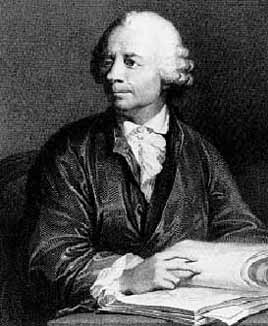
\includegraphics[scale=0.4]{euler01.jpg}\vspc
\small Leonard Euler (1707-1783)
\end{multicols}
}

% Section 1 - Review and Motivation
\section{Review and Motivation}

\subsection{What is a Differential Equation}
\frame{
  \frametitle{What is a Differential Equation? Solution?}

A {\bf differential equation} is an equation which describes a function \vspace{3mm}\\and one or more of its \underline{\hspace{50mm}} of the \vspace{3mm}\\ \underline{\hspace{50mm}}\hspace{3mm}\underline{\hspace{50mm}}\vspace{2mm}\\ with respect to the \underline{\hspace{60mm}}. \vspace{8mm} \\
 
The {\bf solution} to a differential equation describes the \vspace{2mm}\\ \underline{\hspace{40mm}}\hspace{2mm}\underline{\hspace{40mm}} as a function \vspace{2mm}\\of the \underline{\hspace{40mm}}\hspace{2mm}\underline{\hspace{40mm}}.  \vspace{5mm}\\

}

\subsection{Analytical vs. Numerical Solutions}
\frame{

\frametitle{Analytical vs. Numerical Solutions}

\textbf{Analytical}
\begin{itemize}
	\item solution to a problem that can be written in {\bf closed form} 
	\item solution in terms of known functions, constants, etc.  
	\item gives an {\bf exact answer}  \vspcc
\end{itemize}

\textbf{Numerical}
\begin{itemize}
	\item an {\bf approximation} to the solution of a mathematical equation
	\item known as {\bf numerical integration}
	\item numerical integration is more than {\it the computation of integrals}
\end{itemize}

}
 
\subsection{Which one should you choose?}
\frame{
\frametitle{Which one should you choose?}

\scalebox{2}{?\hspc?\hspc?\hspc?\hspc?} \vspcc
 
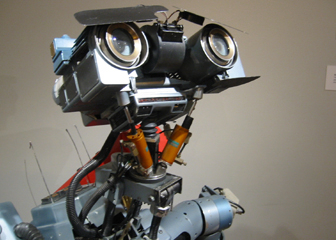
\includegraphics[scale=.3]{johnny5_01.jpg}\vspcc
\scalebox{1.25}{It depends on the problem. It also depends on} \vspc
\scalebox{1.25}{how you intend to use the solution.} \vspcc

}

% Section 2 - Euler's Forward Integration
\section{Euler's Forward Integration}
\subsection{The Initial Value Problem}
\frame{

\frametitle{The Initial Value Problem}

You learned about the {\bf initial value problem} in differential equations class. Do you remember?\vspcc

You have probably been thinking about this idea for much longer than that. Consider riding in a {\it truck} waiting to arrive at you destination...\vspace{10mm}\\
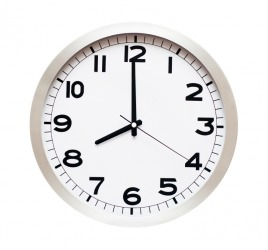
\includegraphics[scale=0.15]{time.jpg}\\
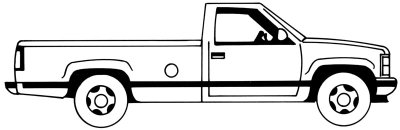
\includegraphics[scale=0.35]{lecture1_fig1.png}

}

\frame{

\frametitle{Integrating a Rate}

You may not have known it but you where {\bf integrating} when performing these mental calculations. You can math.\vspace{20mm}\\

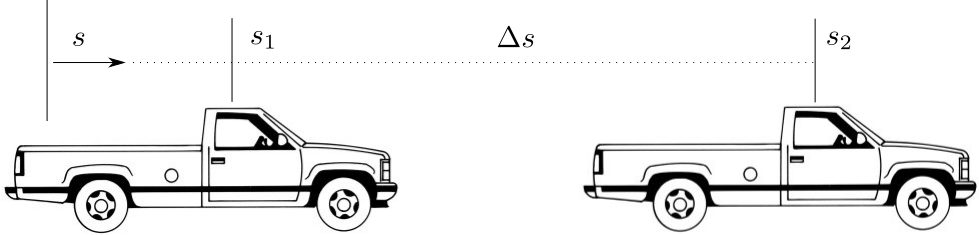
\includegraphics[scale=0.35]{lecture1_fig2.png}

}


\subsection{The Taylor Series}
\frame{
\begin{multicols}{2}
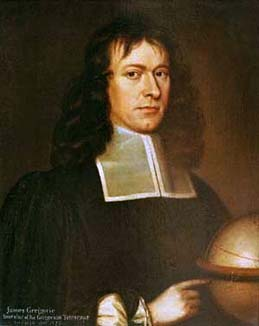
\includegraphics[scale=0.2]{James_Gregory.jpeg}\vspc
\small James Gregory (1638-1675)

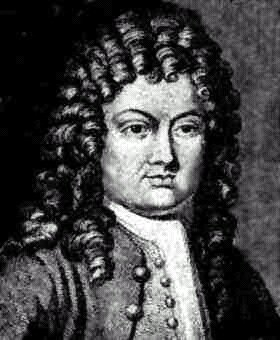
\includegraphics[scale=0.2]{BTaylor.jpg}\vspc
\small Brook  Taylor (1685-1731)
\end{multicols}

\frametitle{The Taylor Series}


Consider the Taylor Series. How does this apply to our problem? \vspc
\scalebox{1}{$y(x)\approx$}\vspc
\scalebox{.9}{$y(a)+y'(a)(x-a)+\frac{y''(a)}{2!}(x-a)^2+\frac{y^{(3)}(a)}{3!}(x-a)^3+...+\frac{y^{(n)}(a)}{n!}(x-a)^n$}\vspc
What does this even mean?
}


\subsection{Euler's Method}
\frame{

\frametitle{Euler's Method}

Given a {\it function describing the slope} and an {\it initial condition}, discretized values of the solution can be approximated. \vspc
This is known as {\bf Euler's method}.\vspccc

	\scalebox{1.0}{$y(x+\Delta x)=y(x) + \frac{dy}{dx}\Delta x=y(x) + f(x,y(x))\Delta x$}\vspcc
	It is commonly shown with subscript notation.\\
	
	\begin{framed}
	\scalebox{1.0}{$y(x_{i+1})=y(x_i) + f(x_i,y(x_i))=y_i + f(x_i,y_i)\Delta x$}\vspcc
	\end{framed}

\small Careful: This is not the same as Euler's formula which is an essential trigonometric identity also used in differential equations.\\

}


\subsection{The Slope Function}
\frame{

\frametitle{The Slope Function}

The differential equation must be written as a function describing the first derivative or {\it the slope} of the dependent variable.\vspc

	\scalebox{1.25}{$f(x,y)=\frac{dy}{dx}\neq y(x)$}\vspcc
	or with subscript notation shown below\vspcc
	\scalebox{1.25}{$f(x_i,y_i)$}\vspcc
	

\small Careful: The first argument $x$ is not always used and is often left out. However it is an important placeholder (ODE45()) and shows this method can be used for {\it non-linear} equations with generalized input functions. 

}

\subsection{Forward Integration}
\frame{

\frametitle{Forward Integration}

Using this concept to solve the initial value problem is called {\bf Euler's forward integration} or {\bf Euler's Method}. Most of the time, the independent variable is \underline{\hspace{30mm}}. \vspcc

Compute the values of the solution one-by-one {\bf forward in time}. \vspcc
\begin{multicols}{2}
\scalebox{1}{$\underline{y(t_{i+1})=y(t_i)+f(t_i,y_i)\Delta t}$}\vspc
\scalebox{1}{$y(\hspccc)=y(\hspccc)+f(\hspccc,\hspccc)\Delta t$}\vspc
\scalebox{1}{$y(\hspccc)=y(\hspccc)+f(\hspccc,\hspccc)\Delta t$}\vspc
\scalebox{1}{$y(\hspccc)=y(\hspccc)+f(\hspccc,\hspccc)\Delta t$}\vspc

\hspace{5mm}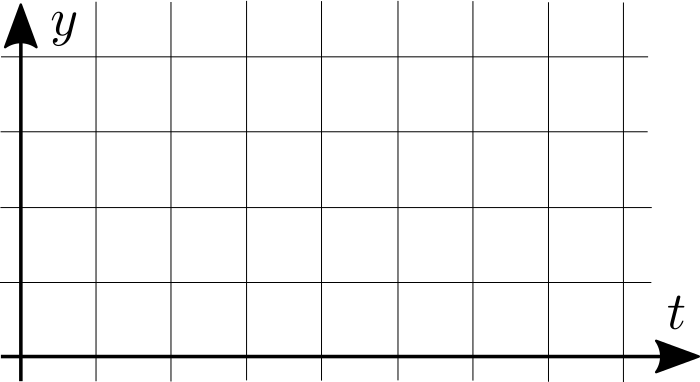
\includegraphics[scale=0.25]{lecture1_fig3.png}
\end{multicols}

}
% Section 4: A Simple Example

\section{A Simple Example}
\frame{

\frametitle{The Previous Example - Radio Flyer}

\begin{multicols}{2}
If this is a valid technique we should be able to solve the problem we solved in the previous lecture. Ferrari anyone? Let's do a Radio Flyer instead. \\ 

\hspace{10mm}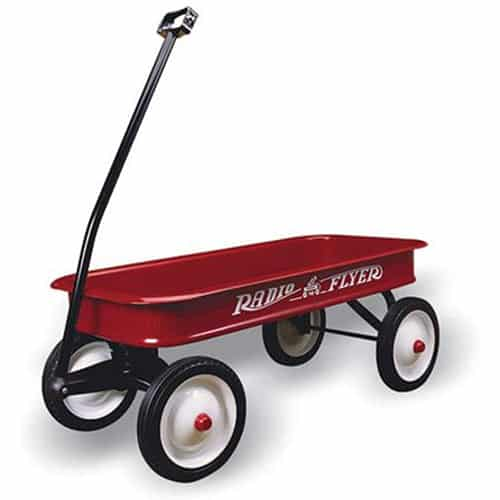
\includegraphics[scale=0.15]{Radio-Flyer.jpg} \vspc

\end{multicols}

\scalebox{1.25}{$m\dot{v}+cv=0 \hspace{3mm} with \hspace{3mm}v(t=0)=v_0$} \vspcc
\scalebox{1.25}{$\hspace{5mm}\implies\hspace{5mm}v(t)=v_0e^{-\frac{c}{m}t}$} \vspace{5mm}\\

}


\frame{

\subsection{The Problem Statement}
\frametitle{The Problem Statement}

This method is not difficult {\it if} we setup  the problem correctly. Read the problem statement carefully.\vspcc

\begin{framed}
Approximate a solution to the differential equation using Euler's Method. Graph the solution from $0$ to $10$ seconds and use a stepsize of $\Delta t=\paramDTA,\hspc\paramDTA,\hspc$and$\hspc \paramDTA $ seconds.\vspcc
\scalebox{1.25}{$m\dot{v}+cv=0 \hspace{3mm} with \hspace{3mm}v(t=0)=v_0$}\vspcc
\scalebox{1.0}{$m=\paramM(kg), \hspc c=\paramC (\frac{n-m}{s}), v_0=\paramVO(\frac{m}{s})$}
\end{framed}

}

\frame{


\frametitle{Breakdown The Problem Statement}
\begin{tabular}{cc}
\underline{ODE:}&\scalebox{1.0}{$m\dot{v}+cv=0$}\vspcc
\underline{Initial Condition:}&\scalebox{1.0}{$\hspace{3mm}v(t=0)=v_0$}\vspcc
\underline{Parameters:}&\scalebox{1.0}{$m=100(kg), \hspc c=0.5 (\frac{n-m}{s}), v_0=5(\frac{m}{s})$}\vspcc
\underline{Strategy:}& Euler's Method, $\Delta t=\paramDTA,\hspc\paramDTB,\hspc$and$\hspc \paramDTC (s) $  \vspccc
\end{tabular}

Look at the formula we derived. What goes where?\vspcc


\scalebox{1.0}{$y_{i+1}=y_i + f(x_i,y_i)\Delta x$}\vspcc
}




\subsection{Execute Euler's Method}

\frame{
\frametitle{Execute Euler's Method}
First, write the {\bf slope function}. \vspc
\scalebox{1}{$f(t,y(t))=f(t,y)=$}\vspc
Then, start with the initial condition and compute the values of the solution {\it one by one, forward in time}. \vspcc

\scalebox{1}{$\underline{v(t_{i+1})=v(t_i)+f(v(t_i))\Delta t}$}\vspc
\scalebox{1}{$v(\hspccc)=v(\hspccc)+f(\hspccc)\Delta t$}\vspc
\scalebox{1}{$v(\hspccc)=v(\hspccc)+f(\hspccc)\Delta t$}\vspc
\scalebox{1}{$v(\hspccc)=v(\hspccc)+f(\hspccc)\Delta t$}\vspc
\scalebox{1}{$v(\hspccc)=v(\hspccc)+f(\hspccc)\Delta t$}\vspc

 This method is not suitable for manual computation. \vspace{0mm}\\

}


% Section 4: MATLAB Solution
\section{MATLAB Solution}

\subsection{Part 1 - Setup and Analytical Solution}
\frame[containsverbatim]{
  \frametitle{Part 1 - Setup and Analytical Solution}



\begin{lstlisting}
% ME 3001 - Mechanical Engineering Analysis
% Tristan Hill - Spring 2020
% Numerical Integration - Lecture 1 
clear variables;close all;clc

% define the constant parameters
m=100;c=1.5;v0=2.0;
dt=1.0;tstop=60;

% create an array of time values
time=0:dt:tstop;
% compute solution from derived equation
v_exact=v0*exp(-c/m*time);
\end{lstlisting}

}

\subsection{Part 2 - Euler's Method}
\frame[containsverbatim]{
  \frametitle{Part 2 - Euler's Method}

% This method is not suitable for manual computation. \vspace{0mm}\\

 \begin{lstlisting}
% approximate with Euler's forward integration
v_eu(1)=v0;
for j=1:length(time)-1
    v_eu(j+1)=v_eu(j)+(f(time(j),v_eu(j),m,c))*dt;  
end

% If this is an 'Inline Definition' of the function 
% it MUST go at the bottom of the script
function [dvdt]=f(t,v,M,C)
    dvdt=-C/M*v;
end

  \end{lstlisting}

}

\subsection{Part 3 - Graph the Solutions}
\frame[containsverbatim]{
  \frametitle{Part 3 - Graph the Solutions}

% This method is not suitable for manual computation. \vspace{0mm}\\

 \begin{lstlisting}
% plot the results of both methods
figure(1);hold on
plot(time,v_exact,'r-','LineWidth',2)
plot(time,v_eu,'b*')

% add some labels
title('Radio Flyer: mdv/dt+cv=0, v(t=0)=v0')
legend('Exact','Euler''s')
xlabel('Time (s)')
ylabel('Velocity')
grid on
  \end{lstlisting}

}


\frame[containsverbatim]{
\frametitle{ Do you believe the results?}

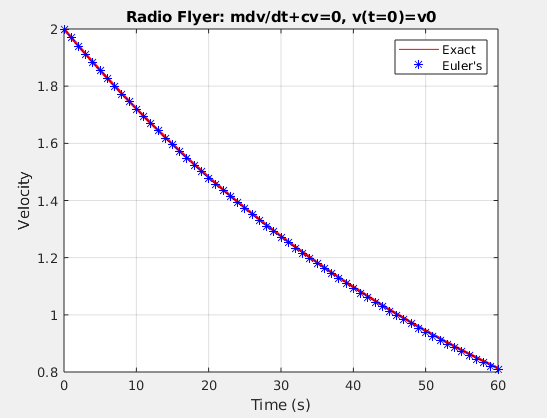
\includegraphics[scale=0.35]{lecture1_fig4.png} \vspc


}


\end{document}









